\section {Complexidade do problema da bissecção}

	Nesta seção apresentaremos a demonstração de que o problema 
	da bissecção mínima é NP-difícil.
	Esse resultado deve-se a Garey, Johnson e Stockmeyer~\cite{GareyJS76},
	e foi obtido através de duas reduções.
	Os autores demonstraram primeiro que o problema {\sc maxcut},
	definido abaixo, é NP-difícil, a partir de uma redução do
	fundamental \textsc {max2sat}, também definido abaixo, e em seguida
	demonstraram que o problema da bissecção mínima é NP-difícil
	a partir de uma redução de {\sc maxcut}.

	Optamos por representar essas duas reduções no TCC.
	Começamos definindo os problemas usados.

	% Nesta seção veremos duas reduções que provam que o problema 
	% da bissecção mínima é NP-Completo~(NP-Difícil 
	% por não ser um problema de decisão),
	% usando o fato de
	% que a versão de decisão do
	% problema {\sc max2sat} é NP-completa.

	% Primeiramente, vamos definir alguns problemas para facilitar
	% a compreensão das reduções.

	\medskip

	\begin{prob}[{\sc max2sat}($C,k$) -- Satisfatibilidade máxima com no máximo 
	dois literais por cláusula]
		Dados um conjunto~$C$ com~$p$ cláusulas distintas na forma 
		normal disjuntiva, com no máximo
		dois literais cada, e um inteiro~${k\le p}$,
		decidir se existem valores para cada uma das variáveis de forma
		que~$k$ ou mais cláusulas de~$C$ sejam verdadeiras.

		%~$C_i=(x_1 x_2)$,
	\end{prob}

	\medskip

	\begin{prob}[{\sc maxcut}($G,W$) -- Corte máximo]
		Dados um grafo~${G}$
		%onde cada uma das arestas tem peso 1, 
		e um inteiro positivo~${W}$, decidir se existe um
		corte~$(T,F)$ em $G$ tal 
		que~${e_G(T,F)\ge W}$.
		
	\end{prob}


	Richard Manning Karp~\cite{Kar72} demonstrou que o problema 
	{\sc max3sat} é NP-difícil,
	e isso foi utilizado por Garey, 
	Johnson e Stockmeyer~\cite{GareyJS76} 
	para provar que 
	o problema {\sc max2sat} é NP-difícil.
	Usaremos esse fato na demonstração do seguinte.


	% \begin{prob}[Corte mínimo em subconjuntos de mesmo tamanho 
	% {~\cite{GareyJS76}}]
	% 	Dado um grafo~$G(V,E)$, onde cada uma das arestas tem 
	% 	peso 1, e um inteiro positivo~$W\le|E|$, encontrar um
	% 	conjunto de vértices~$S\subseteq V$ tal 
	% 	que~$e_G(S,V\setminus~S)\ge W$.
		
	% \end{prob}

	\bigskip
	\bigskip

	\subsection{Redução do \textbf{\textsc {max2sat}} para o \textbf{\textsc {maxcut}}}

		\begin{teo}
			%A instância~$(G,W)$ de {\sc maxcut} tem solução se e somente se
			%a instância~$(C,k)$ de {\sc max2sat} tem solução.
			{\sc maxcut} é NP-difícil.
		\end{teo}
	\begin{proof}
		Vamos apresentar uma redução polinomial do {\sc max2sat}
		para o {\sc maxcut}.

		Dada uma instância~$(C,k)$ do problema {\sc max2sat}, 
		precisamos construir uma instância~$(G,W)$
		do problema {\sc maxcut}, ou seja, um grafo~${G = (V,E)}$
		e um inteiro positivo~$W$.

		% usando a resução que será descrita abaixo.
		%Para isso vamos definir alguns conceitos referentes
		%ao problema {\sc max2sat}:
		%\begin{itemize}
		Seja $p$ o número de cláusulas em~$C$ e
			$n$ o número de variáveis em~$C$.
		Denote por~$x_1,x_2,\ldots,x_n$ as variáveis
		de~$C$.
		Lembre-se que~$\overline{x}$ é a negação da variável~$x$
		e que um literal de~$C$ é uma variável de~$C$ ou a 
		negação de uma variável de~$C$.
		%\end{itemize}

		% A redução consiste em criar um grafo~${G=(V,E)}$, de 
		% acordo com uma entrada para o problema {\sc max2sat}.
		% Segue o conjunto de vértices e arestas de~$G$, 
		% respectivamente.
		O conjunto de vértices de~$G$ é definido da seguinte maneira:
		\begin{align}
			V = \ &\{x_i: 1\le i\le n\} \ \cup \nonumber\\
				&\{\overline{x_i}: 1\le i\le n\} \ \cup\nonumber\\ 
				&\{T_j: 0\le j\le 3p\} \ \cup \nonumber\\
				&\{F_j: 0\le j\le 3p\} \ \cup \nonumber\\
				&\{t_{ij}: 1\le i\le n,\ 0\le j\le 3p\} 
					\ \cup \nonumber\\
				&\{f_{ij}: 1\le i\le n,\ 0\le j\le 3p\}.\nonumber
		\end{align}

		\bigskip 

		O conjunto de arestas de~$G$ é dado em partes. 
		Primeiro, considere
		\begin{align}
			E_1= \ &\{ \{T_i,F_j\}: 0\le i\le 3p,\ 0\le j\le 3p\}\ \cup 
					\nonumber\\
				&\{\{t_{ij}, f_{ij}\}: 1\le i\le n,\ 
					0\le j\le 3p\}\ \cup \nonumber \\
				&\{\{x_i, f_{ij}\}: 1\le i\le n,\ 
					0\le j\le 3p\} \ \cup \nonumber \\
				&\{\{\overline{x_i}, t_{ij}\}: 1\le 
					i\le n,\ 0\le j\le 3p\}. \nonumber
		\end{align}

		\bigskip 

		% \begin{align}
		% 	E_1=&\textcolor{blue}{\{ \{T_i,F_j\}: 0\le i\le 
		% 		3p, 0\le j\le 3p\}} &\cup \nonumber\\
		% 		&\textcolor{green!70}{\{\{t_{ij}, f_{ij}\}: 1\le i\le n, 
		% 			0\le j\le 3p\}} &\cup \nonumber \\
		% 		&\textcolor{brown}{\{\{x_i, f_{ij}\}: 1\le i\le n, 
		% 			0\le j\le 3p\}} &\cup \nonumber \\
		% 		&\textcolor{violet}{\{\{\overline{x_i}, t_{ij}\}: 1\le 
		% 			i\le n, 0\le j\le 3p\}} \nonumber \\
		% \end{align}

		%E para cada uma das~$p$ cláusulas da forma~$C_i=(a_i\lor b_i)$, 
		%temos também as arestas a seguir.

		Agora, sejam~$C_1,C_2,\ldots,C_p$ as cláusulas de~$C$ e sejam~$a_i$
		e~$b_i$ os literais de~$C_i$ para~$i=1,2,\ldots,p$.
		Conseidere então
		\begin{align}
			E_2= \ &\{ \{a_i,b_i\}: 1\le i\le p,\ a_i\ne b_i \}\ \cup 
					\nonumber\\
				&\{\{a_i, F_{2i-1}\}: 1\le i\le p\}\ \cup \nonumber \\
				&\{\{b_i, F_{2i}\}: 1\le i\le p\}. \nonumber
		\end{align}


		Dessa forma, temos o grafo~${G = (V,E)}$, com~${E=E_1\cup E_2}$,
		e o inteiro positivo~${W = |E_1|+2k}$.
		Note que o grafo é simples pois não há cláusulas repetidas em~$C$.

		Segue abaixo um exemplo de grafo~$G$ obtido da
		cláusula~${(x_1\lor\ \overline{x_2})}$.
		%As arestas de~$E_2$ estão representadas pela cor 
		%\textcolor{red}{\textbf {vermelha}}.

		\bigskip

		\begin{center} 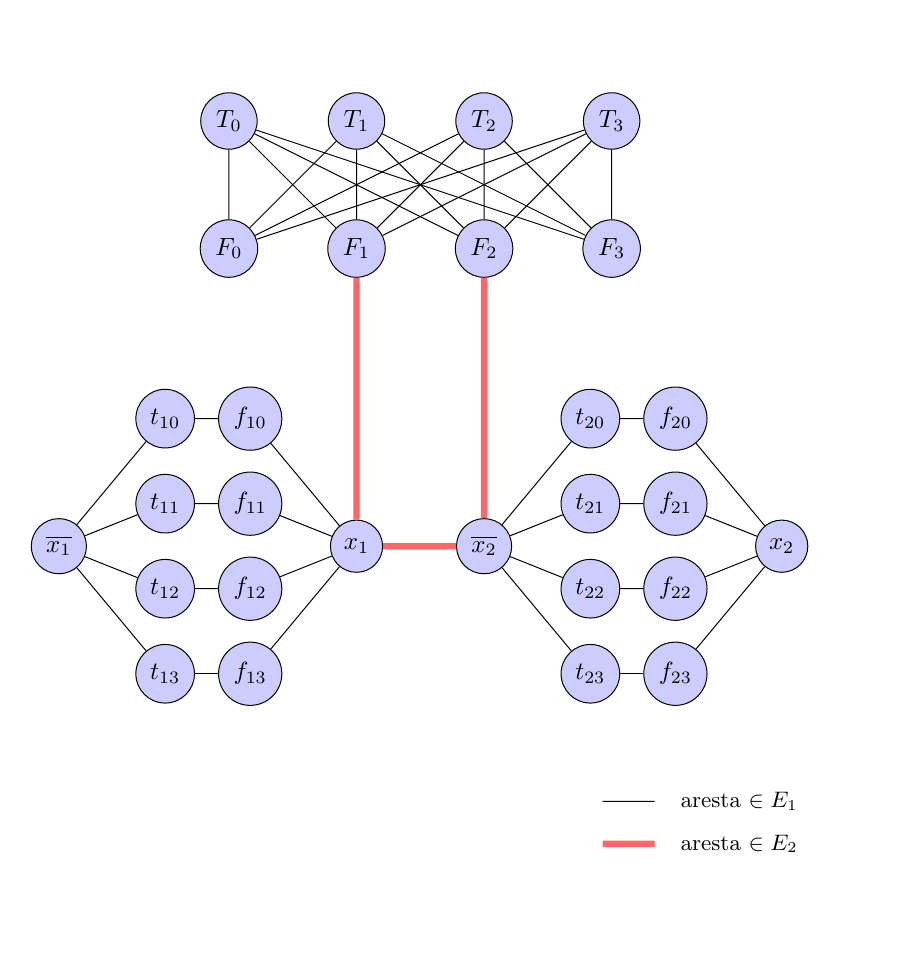
\begin{tikzpicture}
			[scale=.6,auto=left,every node/.style={circle, 
			draw=black,
			fill=blue!20}]
		\scalebox{0.9}{
			\node (t0) at (4, 13)  {$T_0$};
			\node (t1) at (7, 13)  {$T_1$};
			\node (t2) at (10,13)  {$T_2$};
			\node (t3) at (13,13)  {$T_3$};

			\node (f0) at (4, 10)  {$F_0$};
			\node (f1) at (7, 10)  {$F_1$};
			\node (f2) at (10,10)  {$F_2$};
			\node (f3) at (13,10)  {$F_3$};




			\node (t10) at (2.5,6)  {$t_{10}$};
			\node (t11) at (2.5,4)  {$t_{11}$};
			\node (t12) at (2.5,2)  {$t_{12}$};
			\node (t13) at (2.5,0)  {$t_{13}$};	

			\node (f10) at (4.5,6)  {$f_{10}$};
			\node (f11) at (4.5,4)  {$f_{11}$};
			\node (f12) at (4.5,2)  {$f_{12}$};
			\node (f13) at (4.5,0)  {$f_{13}$};
			  
			\node (f20) at (14.5,6)  {$f_{20}$};
			\node (f21) at (14.5,4)  {$f_{21}$};
			\node (f22) at (14.5,2)  {$f_{22}$};
			\node (f23) at (14.5,0)  {$f_{23}$};

			\node (t20) at (12.5,6)  {$t_{20}$};
			\node (t21) at (12.5,4)  {$t_{21}$};
			\node (t22) at (12.5,2)  {$t_{22}$};
			\node (t23) at (12.5,0)  {$t_{23}$};

			
			


			\node (x1n) at (0,3)  {$\overline{x_1}$};
			\node (x1)  at (7,3)  {$x_1$};
			\node (x2n)  at (10,3)  {$\overline{x_2}$};
			\node (x2) at (17,3)  {$x_2$};


			%%legenda
			\node [draw=none, fill=none](a1) at (12.5,-3) {};
			\node [draw=none, fill=none](a1_) at (14.3,-3) {};
			\node [draw=none, fill=none](a2) at (12.5,-4) {};
			\node [draw=none, fill=none](a2_) at (14.3,-4) {};
			\node [draw=none, fill=none] at 
				(16,-3) {\small{aresta $\in E_1$}};
			\node [draw=none, fill=none] at 
				(16,-4) {\small{aresta $\in E_2$}};

			\foreach \from/\to in {t0/f0,t0/f1,t0/f2,t0/f3,
			t1/f0,t1/f1,t1/f2,t1/f3,
			t3/f0,t3/f1,t3/f2,t3/f3,
			t2/f0,t2/f1,t2/f2,t2/f3,a1/a1_}%%%%
			\draw[] (\from) -- (\to);

			\foreach \from/\to in {t10/f10,t11/f11,t12/f12,t13/f13,
			t20/f20,t21/f21,t22/f22,t23/f23}%%%%
			\draw[] (\from) -- (\to);

			\foreach \from/\to in {t10/x1n,t11/x1n,t12/x1n,t13/x1n,
			t20/x2n,t21/x2n,t22/x2n,t23/x2n}
			\draw[] (\from) -- (\to);

			\foreach \from/\to in {x1/f10,x1/f11,x1/f12,x1/f13,
			x2/f20,x2/f21,x2/f22,x2/f23}
			\draw[] (\from) -- (\to);

			\foreach \from/\to in {x1/x2n,x1/f1,x2n/f2,a2/a2_}
			\draw[draw=red!60, line width=2.5pt] (\from) -- (\to);
		}
		\end{tikzpicture} \end{center}
		Claramente~$G$ e~$W$ podem ser obtidos de~$(C,k)$ em
		tempo polinomial em~$p$ e~$n$.
		Resta mostrar que existe uma atribuição de valores para as
		variáveis de~$C$ que satisfaz pelo menos~$k$ cláusulas de~$C$
		se e somente se existe um corte~$(T,F)$ em~$G$ tal 
		que~$e_G(T,F)\ge W$.


		%Provaremos agora que a instância~$(G,W)$ de {\sc maxcut} tem solução se
		%a instância~$(C,k)$ de {\sc max2sat} tem solução.
		%para todas as entradas do problema
		%{\sc max2sat}, existe uma solução da sua redução para o problema
		%{\sc maxcut}.
		
		%Sabe-se que temos um conjunto de cláusulas~$C$
		%de forma que~$k$ ou mais
		%cláusulas sejam verdadeiras.
		\bigskip
		\bigskip

		Agora vamos supor que temos um conjunto de valores para 
		as variáveis de~$C$ que tornam~$k$ ou mais cláusulas
		de~$C$ verdadeiras.

		Note que existem no máximo~$2p$ arestas do 
		tipo~${\{x_i,F_j\}}$ ou ${\{\overline{x_i},F_j\}}$. 
		Dado que~${2p<3p+1}$ e
		as funções~${f(i)=2i - 1}$ e~${g(i)=2i}$ têm 
		imagens disjuntas e são injetoras, 
		temos que cada~$F_j$ se liga a apenas um vértice
		do tipo~$x_i$ ou~${\overline{x_i}}$.

		Definiremos agora os
		conjuntos~$T$ e~$F$ de um corte~$(T,F)$ de~$G$.
		Para todo~${i\in[0,3p]}$,~${T_i\in T}$ 
		e~${F_i\in F}$ e,
		para todo~${j\in[1,n]}$ e ${k\in[0,3p]}$, ~$x_j$ pertence ao 
		mesmo conjunto que~$t_{jk}$ e ambos não pertencem ao mesmo 
		conjunto que~$\overline{x_j}$ e que~$f_{jk}$.
		Assim sendo, todas as arestas de~$E_1$ estão no 
		corte~$(T,F)$.
		Ademais, se a variável~$x_i$ é verdadeira,
		então o vértice~$x_i$ está em $T$, caso contrário,~$x_i$
		está em~$F$.
		%e se mantermos as 
		%propriedades que foram citadas anteriormente, 
		Isso não contraria as escolhas feitas anteriormente, portanto 
		obtemos um corte~$(T,F)$.
		%afetará o 
		%fato de todas as arestas de~$E_1$ estarem no corte~$(T,F)$.
		%Portanto, assumiremos inicialmente que essa é a disposição dos 
		%vértices nos subconjuntos~$T$ e~$F$.

		Em uma cláusula~${C_i=(a_i,b_i)}$, ou
		apenas um dos literais é verdadeiro, ou ambos são, ou nenhum
		deles é.
		\begin{enumerate}
			\item Se apenas um dos literais é verdadeiro,
			das três arestas formadas pela 
			cláusula~$C_i$,~$\{a_i,b_i\}$,~$\{a_i, F_{2i-1}\}$
			e~$\{b_i, F_{2i}\}$, duas delas
			estão no corte~$(T,F)$ e uma está fora.
			\item Se os dois literais são verdadeiros, também teremos
			duas arestas no corte~$(T,F)$ e uma fora.
			\item Já no caso de nenhum literal ser verdadeiro, nenhuma
			dessas arestas da cláusula estará no corte~$(T,F)$.
		\end{enumerate}

		Podemos ver isso de forma mais clara na imagem a seguir.

		\begin{center} 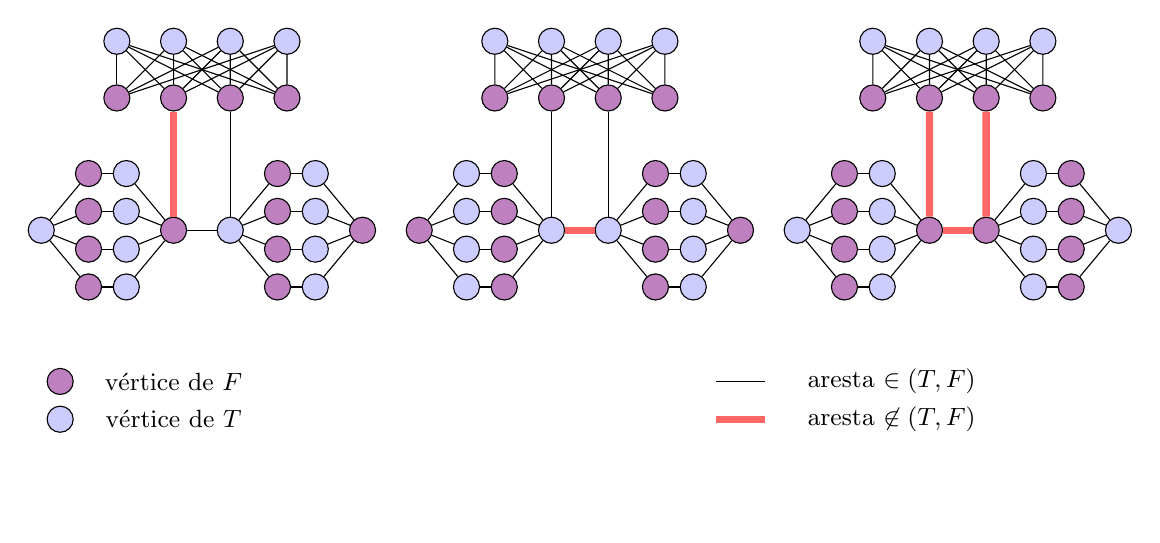
\begin{tikzpicture}
			[scale=.24,auto=left,every node/.style={circle, 
			draw=black,
			fill=blue!20}]
			


			\node (t0_) at (4 +20,13)  {};
			\node (t1_) at (7 +20,13)  {};
			\node (t2_) at (10+20,13)  {};
			\node (t3_) at (13+20,13)  {};

			\node [fill=violet!50](f0_) at (4 +20,10)  {};
			\node [fill=violet!50](f1_) at (7 +20,10)  {};
			\node [fill=violet!50](f2_) at (10+20,10)  {};
			\node [fill=violet!50](f3_) at (13+20,10)  {};

			\node (t10_) at (2.5+20,6)  {};
			\node (t11_) at (2.5+20,4)  {};
			\node (t12_) at (2.5+20,2)  {};
			\node (t13_) at (2.5+20,0)  {};	

			\node [fill=violet!50](f10_) at (4.5+20,6)  {};
			\node [fill=violet!50](f11_) at (4.5+20,4)  {};
			\node [fill=violet!50](f12_) at (4.5+20,2)  {};
			\node [fill=violet!50](f13_) at (4.5+20,0)  {};
			  
			\node (f20_) at (14.5+20,6)  {};
			\node (f21_) at (14.5+20,4)  {};
			\node (f22_) at (14.5+20,2)  {};
			\node (f23_) at (14.5+20,0)  {};

			\node [fill=violet!50](t20_) at (12.5+20,6)  {};
			\node [fill=violet!50](t21_) at (12.5+20,4)  {};
			\node [fill=violet!50](t22_) at (12.5+20,2)  {};
			\node [fill=violet!50](t23_) at (12.5+20,0)  {};
			
			\node [fill=violet!50](x1n_) at (0 +20, 3)  {};
			\node (x1_)  at (7 +20, 3)  {};
			\node (x2n_) at (10+20, 3) {};
			\node [fill=violet!50](x2_)  at (17+20, 3) {};






			\node (t0__) at (4 +40,13)  {};
			\node (t1__) at (7 +40,13)  {};
			\node (t2__) at (10+40,13)  {};
			\node (t3__) at (13+40,13)  {};

			\node [fill=violet!50](f0__) at (4 +40,10)  {};
			\node [fill=violet!50](f1__) at (7 +40,10)  {};
			\node [fill=violet!50](f2__) at (10+40,10)  {};
			\node [fill=violet!50](f3__) at (13+40,10)  {};

			\node [fill=violet!50](t10__) at (2.5+40,6)  {};
			\node [fill=violet!50](t11__) at (2.5+40,4)  {};
			\node [fill=violet!50](t12__) at (2.5+40,2)  {};
			\node [fill=violet!50](t13__) at (2.5+40,0)  {};	

			\node (f10__) at (4.5+40,6)  {};
			\node (f11__) at (4.5+40,4)  {};
			\node (f12__) at (4.5+40,2)  {};
			\node (f13__) at (4.5+40,0)  {};
			  
			\node [fill=violet!50](f20__) at (14.5+40,6)  {};
			\node [fill=violet!50](f21__) at (14.5+40,4)  {};
			\node [fill=violet!50](f22__) at (14.5+40,2)  {};
			\node [fill=violet!50](f23__) at (14.5+40,0)  {};

			\node (t20__) at (12.5+40,6)  {};
			\node (t21__) at (12.5+40,4)  {};
			\node (t22__) at (12.5+40,2)  {};
			\node (t23__) at (12.5+40,0)  {};
			
			\node (x1n__) at (0 +40, 3)  {};
			\node [fill=violet!50](x1__)  at (7 +40, 3)  {};
			\node [fill=violet!50](x2n__) at (10+40, 3) {};
			\node (x2__)  at (17+40, 3) {};






			\node (t0) at (4 ,13)  {};
			\node (t1) at (7 ,13)  {};
			\node (t2) at (10,13)  {};
			\node (t3) at (13,13)  {};

			\node [fill=violet!50](f0) at (4 ,10)  {};
			\node [fill=violet!50](f1) at (7 ,10)  {};
			\node [fill=violet!50](f2) at (10,10)  {};
			\node [fill=violet!50](f3) at (13,10)  {};



			\node [fill=violet!50](t10) at (2.5,6)  {};
			\node [fill=violet!50](t11) at (2.5,4)  {};
			\node [fill=violet!50](t12) at (2.5,2)  {};
			\node [fill=violet!50](t13) at (2.5,0)  {};	

			\node (f10) at (4.5,6)  {};
			\node (f11) at (4.5,4)  {};
			\node (f12) at (4.5,2)  {};
			\node (f13) at (4.5,0)  {};
			  
			\node (f20) at (14.5,6)  {};
			\node (f21) at (14.5,4)  {};
			\node (f22) at (14.5,2)  {};
			\node (f23) at (14.5,0)  {};

			\node [fill=violet!50](t20) at (12.5,6)  {};
			\node [fill=violet!50](t21) at (12.5,4)  {};
			\node [fill=violet!50](t22) at (12.5,2)  {};
			\node [fill=violet!50](t23) at (12.5,0)  {};


			\node (x1n) at (0,3)  {};
			\node [fill=violet!50](x1)  at (7,3)  {};
			\node (x2n) at (10,3) {};
			\node [fill=violet!50](x2)  at (17,3) {};



			\node (l1) at (1,-7)  {};
			\node [fill=violet!50](l2)  at (1,-5)  {};
			\node [draw=none, fill=none] at 
				(7,-5) {\small{vértice de $F$}};
			\node [draw=none, fill=none] at 
				(7,-7) {\small{vértice de $T$}};
			\node [draw=none, fill=none](a1) at (35,-5) {};
			\node [draw=none, fill=none](a1_) at (39,-5) {};
			\node [draw=none, fill=none](a2) at (35,-7) {};
			\node [draw=none, fill=none](a2_) at (39,-7) {};
			\node [draw=none, fill=none] at 
				(45,-5) {\small{aresta $\in(T,F)$}};
			\node [draw=none, fill=none] at 
				(45,-7) {\small{aresta $\not\in(T,F)$}};
			\foreach \from/\to in {t0_/f0_,t0_/f1_,t0_/f2_,t0_/f3_,
			t1_/f0_,t1_/f1_,t1_/f2_,t1_/f3_,
			t3_/f0_,t3_/f1_,t3_/f2_,t3_/f3_,
			t2_/f0_,t2_/f1_,t2_/f2_,t2_/f3_}%%%%
			\draw[] (\from) -- (\to);

			\foreach \from/\to in 
			{t10_/f10_,t11_/f11_,t12_/f12_,t13_/f13_,
			t20_/f20_,t21_/f21_,t22_/f22_,t23_/f23_}%%%%
			\draw[] (\from) -- (\to);

			\foreach \from/\to in 
			{t10_/x1n_,t11_/x1n_,t12_/x1n_,t13_/x1n_,
			t20_/x2n_,t21_/x2n_,t22_/x2n_,t23_/x2n_}
			\draw[] (\from) -- (\to);

			\foreach \from/\to in 
			{x1_/f10_,x1_/f11_,x1_/f12_,x1_/f13_,
			x2_/f20_,x2_/f21_,x2_/f22_,x2_/f23_,x1_/f1_,x2n_/f2_}
			\draw[] (\from) -- (\to);

			\foreach \from/\to in {x1_/x2n_}
			\draw[draw=red!60, line width=2.7pt] (\from) -- (\to);


			

			\foreach \from/\to in {t0__/f0__,t0__/f1__,t0__/f2__,t0__/f3__,
			t1__/f0__,t1__/f1__,t1__/f2__,t1__/f3__,
			t3__/f0__,t3__/f1__,t3__/f2__,t3__/f3__,
			t2__/f0__,t2__/f1__,t2__/f2__,t2__/f3__}%%%%
			\draw[] (\from) -- (\to);

			\foreach \from/\to in 
			{t10__/f10__,t11__/f11__,t12__/f12__,t13__/f13__,
			t20__/f20__,t21__/f21__,t22__/f22__,t23__/f23__}%%%%
			\draw[] (\from) -- (\to);

			\foreach \from/\to in 
			{t10__/x1n__,t11__/x1n__,t12__/x1n__,t13__/x1n__,
			t20__/x2n__,t21__/x2n__,t22__/x2n__,t23__/x2n__}
			\draw[] (\from) -- (\to);

			\foreach \from/\to in 
			{x1__/f10__,x1__/f11__,x1__/f12__,x1__/f13__,
			x2__/f20__,x2__/f21__,x2__/f22__,x2__/f23__,a1/a1_}
			\draw[] (\from) -- (\to);

			\foreach \from/\to in {x1__/x2n__,x1__/f1__,x2n__/f2__,a2/a2_}
			\draw[draw=red!60, line width=2.7pt] (\from) -- (\to);




			\foreach \from/\to in {t0/f0,t0/f1,t0/f2,t0/f3,
			t1/f0,t1/f1,t1/f2,t1/f3,
			t3/f0,t3/f1,t3/f2,t3/f3,
			t2/f0,t2/f1,t2/f2,t2/f3}%%%%
			\draw[] (\from) -- (\to);

			\foreach \from/\to in {t10/f10,t11/f11,t12/f12,t13/f13,
			t20/f20,t21/f21,t22/f22,t23/f23}%%%%
			\draw[] (\from) -- (\to);

			\foreach \from/\to in {t10/x1n,t11/x1n,t12/x1n,t13/x1n,
			t20/x2n,t21/x2n,t22/x2n,t23/x2n}
			\draw[] (\from) -- (\to);

			\foreach \from/\to in {x1/f10,x1/f11,x1/f12,x1/f13,
			x2/f20,x2/f21,x2/f22,x2/f23,x2n/f2,x1/x2n}
			\draw[] (\from) -- (\to);

			\foreach \from/\to in {x1/f1}
			\draw[draw=red!60, line width=2.7pt] (\from) -- (\to);
		\end{tikzpicture} \end{center}
		Note que temos~$2k$ ou mais arestas de~$E_2$ no
		corte~$(T,F)$, pois, para cada uma das~$k$ cláusulas
		verdadeiras, teremos duas arestas de~$E_2$ diferentes no corte, 
		como mostrado anteriormente.
		Portanto, no mínimo~$|E_1| + 2k$ arestas de~$G$ estão no corte~$(T,F)$.

		% Se houvesse alguma aresta duplicada (duas arestas que ligam
		% os mesmos vértices), teríamos um problema na contagem de
		% arestas dentro e fora do corte.
		% Isso poderia ocorrer no caso de duas cláusulas serem 
		% idênticas,~${C_i=C_j=(a_i,b_i)}$.
		% Isso faria com que houvesse uma aresta duplicada entre
		% os vértices~$a_1$ e~$b_i$, mas isso não acontece, dado que
		% no enunciado é assumido que as cláusulas são distintas.
		% Também não há o problema de dois vértices estarem em cláusulas
		% diferentes, dado que para cada cláusula, os vértices se ligam
		% a um~$F_i$ diferente.
		% E mesmo se repetirmos as variáveis na mesma cláusula, cada
		% elemento da cláusula se ligará a um~$F_i$ diferente.

		% \bigskip

		% Mostramos que existe uma solução, em {\sc maxcut}, 
		% para todas as entradas do
		% problema {\sc max2sat} reduzidas para {\sc maxcut}, de forma que
		% a solução do {\sc maxcut} leva a uma solução de {\sc max2sat}.
		% Agora mostraremos que qualquer solução obtida em 
		% uma redução para {\sc maxcut} levará a uma solução de {\sc max2sat}.

		\bigskip
		\bigskip

		
		Agora vamos supor que temos uma instância~$(G,W)$,
		com~$G=(V,E)$, obtida através da redução de uma instância~$(C,k)$.
		Seja~$(T,F)$ um corte em~$G$,
		com~$e_G(T,F)\ge W$.
		Temos que provar que
		existem no mínimo~$k$ cláusulas verdadeiras em~$C$.

		% Sabemos que existem~$3p+1$ vértices do tipo~$T_j$
		% e~$3p+1$ vértices do tipo~$F_j$, e 
		% existem também arestas que ligam todos os vértices
		% de~$T_j$ a todos os vértices de~$F_j$, mas nenhuma
		% delas liga .
		Note que, como o conjunto~$E_2$ é composto por três arestas
		de cada uma das cláusula de~$C$,~${|E_2| = 3}p$.  
		Se os vertices do tipo~$T_j$ e os do tipo~$F_j$ não
		ficarem separados no corte~$(T,F)$,
		no mínimo~${3p+1}$ arestas de~$E_1$ não estarão
		no corte~$(T,F)$ e, 
		consequentemente,~${e_G(T,F)\le |E_1|-(3p+1)+|E_2|< |E_1| \le W}$. 
		Portanto, os vértices do tipo~$T_j$ e~$F_j$
		estão em conjuntos diferentes no corte~$(T,F)$
		e todas as arestas do tipo~$\{T_i,F_j\}$ estão no
		corte~$(T,F)$.

		De maneira similar, podemos ver que para toda 
		variável~$x_i$, os vértices~$x_i$ e~$\overline{x_i}$
		de~$V$ estão em conjuntos diferentes no corte~$(T,F)$.
		Existem~$3p+1$ caminhos diferentes entre~$x_i$
		e~$\overline{x_i}$, e cada um deles contém~4
		vértices~${(x_i,\ f_{ij},\ t_{ij} \ \text{e}\ \overline{x_i})}$.
		Se~$x_i$ pertence ao mesmo conjunto que~$\overline{x_i}$,
		pelo menos uma aresta de cada caminho não estará contida
		no corte~$(T,F)$, ou seja, no mínimo~$3p+1$ arestas
		de~$E_1$ não estarão no corte~$(T,F)$, o que
		implica que~${e_G(T,F)< W}$, como visto anteriormente.

		Os vértices do tipo~$t_{ij}$ e~$f_{ij}$ servem unicamente
		para que~$x_i$ e~$\overline{x_i}$ fiquem em conjuntos
		diferentes no corte~$(T,F)$.
		O ideal seria que estes vértices fossem dispostos no 
		corte~$(T,F)$ de forma que todas as arestas de~$E_1$ 
		estivessem no corte~$(T,F)$, assim no mínimo~$2k$ arestas 
		de~$E_2$ estariam em~$(T,F)$.
		Mas, se isso não ocorrer,
		o número de arestas de~$E_2$ irá suprir a falta de arestas
		de~$E_1$ no corte,
		fazendo com que o número de cláusulas verdadeiras seja maior
		que~$2k$.
		Portanto, não importa em quais conjuntos do corte~$(T,F)$ os 
		vértices do tipo~$t_{ij}$ e~$f_{ij}$ estão.

		Como todos os vértices do tipo~$F_i$ estão no mesmo conjunto
		do corte~$(T,F)$, e sabendo que cada cláusula gera um 
		caminho do tipo~$F_m,x_n,x_o,F_p$, somente será possível
		dispor os vértices do grafo de forma que, para cada cláusula,
		zero (cláusula falsa) ou duas (cláusula verdadeira) arestas 
		estejam no corte~$(B,W)$.
		Dessa forma, no mínimo~$k$ cláusulas serão verdadeiras. 

		Seja~$F$ o conjunto do corte~$(T,F)$ onde estão todos os vértices
		da forma~$F_i$.
		Uma cláusula é verdadeira quando dois de seus vértices
		estão no corte~$(T,F)$, então os literais com valor verdadeiro
		devem estar no conjunto~$T$,
		ou seja, 
		se o vértice~$x_i\in T$, a variável~$x_i$ tem valor verdadeiro.
		Caso contrário,~$\overline{x_i}\in T$ e a variável~$x_i$ tem valor falso.
		
		Os valores das variáveis de~$C$ podem ser obtidos de~$G$ em
		tempo polinomial em~$n$.
	\end{proof}


		% Caso algum desses vértices não esteja conforme o especificado
		% na redução, o número de arestas de~$E_1$
		% no corte vai ser menor, o que faz com que o valor de~$W$ seja 
		% compensado pelo número de arestas de~$E_2$ no corte.
		% Logo, caso algum vértice de 


		% Se existe um corte~$(T,F)$ em~$G$ tal 
		% que~${e_G(T, F)\ge W}$, 
		% então teremos que, para todo vértice do tipo~$x_i$,
		% se~${x_i\in T}$, a variável que ele representa terá valor
		% verdadeiro. 
		% Caso contrário,~${x_i\in F}$ e a variável que ele 
		% representa terá valor falso. 
		% Note que, para essa valoração das variáveis de~$C$,
		% pelo menos~$k$ cláusulas de~$C$ são satisfeitas.


		%Tendo que as variáveis possuem os valores conforme
		%o que foi dito anteriormente, $k$ ou mais cláusulas serão 
		%verdadeiras.
	%\end{proof}


	\bigskip
%%%%%%%%%%%%%%%%%%%%%%%%%%%%%%%%%%%%%%%%%%%%%%%%%%%%%%%%%%%%%%%%%%%%%%%%
%%%%%%%%%%%%%%%%%%%%%%%%%%%%%%%%%%%%%%%%%%%%%%%%%%%%%%%%%%%%%%%%%%%%%%%%
%%%%%%%%%%%%%%%%%%%%%%%%%%%%%%%%%%%%%%%%%%%%%%%%%%%%%%%%%%%%%%%%%%%%%%%%


\subsection{Redução do \textbf{\textsc{maxcut}} para a Bissecção}
	\begin{prob}[Bissecção($G,W$) -- Corte mínimo em uma bissecção]
		Dados um grafo~${G}$
		%onde cada uma das arestas tem peso 1, 
		e um inteiro positivo~${W}$, decidir se existe um
		corte~$(R,S)$ em $G$ tal 
		que~$|R|=|S|$ e~${e_G(R,S)\le W}$.
		
	\end{prob}
	\begin{teo}
		O problema da bissecção mínima é NP-difícil.
	\end{teo}
	\begin{proof}
		Vamos apresentar uma redução polinomial do {\textsc{maxcut}}
		para o problema da Bissecção.

		Dada uma instância~$(G,W)$ do problema {\textsc{maxcut}},
		com~${G = (V,E)}$, precisamos construir uma instância~$(G',W')$
		do problema da Bissecção, com~${G'=(V',E')}$.

		Seja~${n = |V|}$ e~${U=\{u_1,u_2,\ldots,u_n\}}$ 
		com~${V\cap U = \emptyset}$.
		O conjunto de vértices e arestas de~$G$ é dado da seguinte 
		maneira:
		\begin{align} 
			V' &= V\cup U \nonumber \\
			E' &= \{\{x,y\}: x,y\in V'\ \ \text{e}\ \ \{x,y\}\not\in E\} \nonumber \\
			W' &= n^2-W .\nonumber 
		\end{align}
		Segue abaixo um exemplo de grafo~$G'$.
\begin{center} 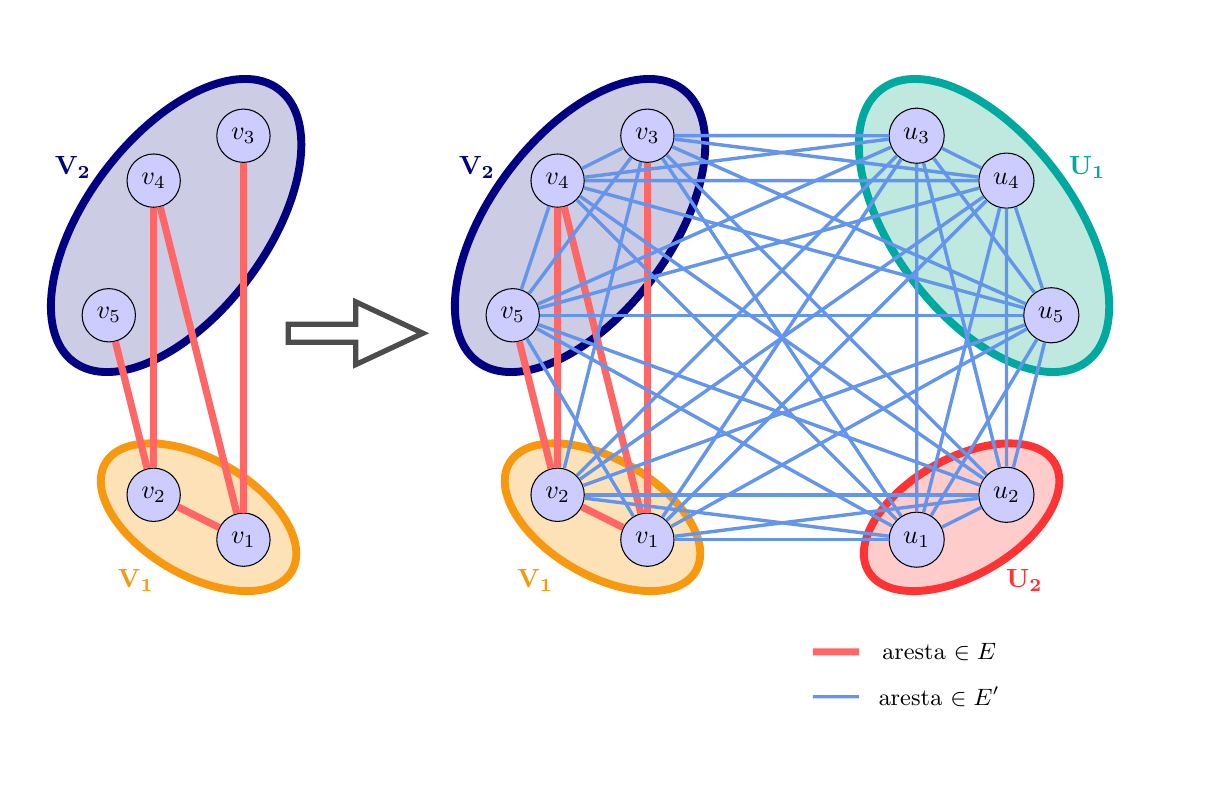
\begin{tikzpicture}
	[scale=.6,auto=left,every node/.style={circle, 
	draw=black,
	fill=blue!20}]
	\scalebox{0.95}{

	\draw [rotate around={60:(-13+15.8,1.5)}, draw=YellowOrange, fill=YellowOrange!25,line width=3pt] (-13+15.8,1.5) 
		ellipse (1.3cm and 2.4cm);
	\draw [rotate around={143:(-13.5+15.8,8)}, draw=NavyBlue, fill=NavyBlue!20,line width=3pt] (-13.5+15.8,8) 
		ellipse (2cm and 3.8cm);
	



	\draw [rotate around={60:(-4+15.8,1.5)}, draw=YellowOrange, fill=YellowOrange!25,line width=3pt] (-4+15.8,1.5) 
		ellipse (1.3cm and 2.4cm);
	\draw [rotate around={143:(-4.5+15.8,8)}, draw=NavyBlue, fill=NavyBlue!20,line width=3pt] (-4.5+15.8,8) 
		ellipse (2cm and 3.8cm);




	\draw [rotate around={-60:(4+15.8,1.5)}, draw=red!80, fill=red!20,line width=3pt] (4+15.8,1.5) 
		ellipse (1.3cm and 2.4cm);
	\draw [rotate around={-143:(4.5+15.8,8)}, draw=Emerald, fill=Emerald!25,line width=3pt] (4.5+15.8,8) 
		ellipse (2cm and 3.8cm);
	

	\node [text=YellowOrange,draw=none, fill=none] at (-14.4+15.8,0.1){$\mathbf{V_1}$};
	\node [text=NavyBlue,draw=none, fill=none] at (-15.8+15.8,9.3){$\mathbf{V_2}$};

	\node [text=YellowOrange,draw=none, fill=none] at (-5.5+15.8,0.1){$\mathbf{V_1}$};
	\node [text=NavyBlue,draw=none, fill=none] at (-6.8+15.8,9.3){$\mathbf{V_2}$};


	\node [text=red!80,draw=none, fill=none] at (5.4+15.8,0.1){$\mathbf{U_2}$};
	\node [text=Emerald,draw=none, fill=none] at (6.8+15.8,9.3){$\mathbf{U_1}$};

	\node (an1) at (-12+15.8, 1) {$v_1$};
	\node (an2) at (-14+15.8, 2) {$v_2$};
	\node (an3) at (-12+15.8, 10) {$v_3$};
	\node (an4) at (-14+15.8, 9) {$v_4$};
	\node (an5) at (-15+15.8, 6) {$v_5$};

	\node (v1) at (-3+15.8, 1)  {$v_1$};
	\node (v2) at (-5+15.8, 2)  {$v_2$};
	\node (v3) at (-3+15.8, 10) {$v_3$};
	\node (v4) at (-5+15.8, 9)  {$v_4$};
	\node (v5) at (-6+15.8, 6)  {$v_5$};

	\node (u1) at (3+15.8, 1)  {$u_1$};
	\node (u2) at (5+15.8, 2)  {$u_2$};
	\node (u3) at (3+15.8, 10) {$u_3$};
	\node (u4) at (5+15.8, 9)  {$u_4$};
	\node (u5) at (6+15.8, 6)  {$u_5$};

	%legenda
	\node [draw=none, fill=none](a1)  at (2  +15.8,-1.5) {};
	\node [draw=none, fill=none](a1_) at (0.4+15.8,-1.5) {};
	\node [draw=none, fill=none](a2)  at (2  +15.8,-2.5) {};
	\node [draw=none, fill=none](a2_) at (0.4+15.8,-2.5) {};

	\node [draw=none, fill=none] at 
		(3.5+15.8,-1.5) {\small{aresta $\in E$}};
	\node [draw=none, fill=none] at 
		(3.5+15.8,-2.5) {\small{aresta $\in E'$}};
	

	\foreach \from/\to in {v1/v4,v1/v2,v1/v3,v2/v4,v2/v5,
	a1/a1_,
	an1/an4,an1/an2,an1/an3,an2/an4,an2/an5}
	\draw[draw=red!60, line width=2.7pt] (\from) -- (\to);

	\foreach \from/\to in {v1/v5,v2/v3,v3/v4,v3/v5,v4/v5,
	u1/u2,u1/u3,u1/u4,u1/u5,u2/u3,u2/u4,u2/u5,u3/u4,u3/u5,u4/u5,
	v1/u1, v1/u2, v1/u3, v1/u4, v1/u5,
	v2/u1, v2/u2, v2/u3, v2/u4, v2/u5,
	v3/u1, v3/u2, v3/u3, v3/u4, v3/u5,
	v4/u1, v4/u2, v4/u3, v4/u4, v4/u5,
	v5/u1, v5/u2, v5/u3, v5/u4, v5/u5,
	a2/a2_}
	%an1/an5,an2/an3,an3/an4,an3/an5,an4/an5}
	\draw[draw=CornflowerBlue,line width=1.3pt] (\from) -- (\to);

	\draw [draw=black!70, line width=2pt]
		(-11.+15.8 ,5.4) -- 
		(-11.+15.8 ,5.8) --
		(-9.5+15.8 ,5.8) --
		(-9.5+15.8 ,6.3) --
		(-8. +15.8 ,5.6) --%%%
		(-9.5+15.8 ,4.9) --
		(-9.5+15.8 ,5.4) --
		cycle;
}
\end{tikzpicture}\end{center}
		Note que~$G'$ e~$W'$ podem ser obtidos de~$G$ e~$W$
		em tempo polinomial em~$n$.	

		\bigskip

		%Agora mostraremos que, para cada instância~$(G,W)$ 
		%de {\sc maxcut}, existe uma instância~$(G',W')$ que
		Agora vamos supor que temos um grafo~$G$ tal que exista um
		corte~$(V_1,V_2)$ em~$G$, onde~$e_G(V_1,V_2)\ge W$.

		%Sejam~$S_1\subset V'$ e~$S_2\subset V'$ tal que~$S_1\cup S_2 = V'$
		Denotemos por~${U_1\subset U}$ e~${U_2\subset U}$ dois conjuntos de vértices
		arbitrários, 
		%escolhidos arbitrariamente,
		tais que~${|U_1| = |V_2|}$,~${|U_2| = |V_1|}$ e~$U_1\cap U_2 = \emptyset$,
		como o ilustrado na figura acima.
		Seja~$(S_1,S_2)$ um corte de~$G'$ tal que~${S_1=V_1\cup U_1}$
		e~${S_2=V_2\cup U_2}$. 
		Note que o corte~$(S_1,S_2)$ é uma bissecção, dado 
		que~${|S_1| = |V_1| + |U_1| = |U_2|+|V_2| = |S_2|}$.

		Se~$G'$ fosse um grafo completo,~$e_{G'}(S_1,S_2) = n^2$,
		mas~$G'$ não é completo, dado que as arestas do corte~$(V_1,V_2)$
		em~$G$ não estão presentes em~$G'$.
		Portanto,~${e_{G'}(S_1,S_2) = n^2 - e_G(V_1,V_2)\le n^2-W}$.

		Podemos concluir que existe um corte~$(S_1,S_2)$ em~$G'$ tal que~${|S_1|=|S_2|}$ 
		e~${e_{G'}(S_1,S_2)\le W'}$.

		\bigskip

		Agora vamos supor que temos uma instância~$(G',W')$, com~${G'=(V',E')}$,
		obtida através da redução de uma instância~$(G,W)$ de {\sc maxcut}, 
		com~${G=(V,E)}$.
		Seja~$(S_1,S_2)$ um corte em~$G'$, com~${e_{G'}(S_1,S_2)\le W'}$ 
		e~${|S_1| = |S_2|}$.
		Temos que provar que existe um corte~$(V_1,V_2)$ em~$G$ tal 
		que~$e_G(V_1,V_2)\ge W$.

		Seja~${V_1 = S_1\cap V}$,~${V_2 = S_2\cap V}$
		%~${U_1 = S_1\setminus V_1}$ e~${U_2 = S_2\setminus V_2}$.
		e~$k$ um inteiro positivo tal que~${e_G(V_1,V_2) = k}$. 
		Se o grafo~$G'$ fosse completo,~${e_{G'}(S_1,S_2) = n^2}$,
		mas como as arestas de~$E$ não estão presentes em~$E'$,
		então~${e_{G'}(S_1, S_2) = n^2 - k}$.

		Dado que~$e_{G'}(S_1,S_2)\le W'$ e que~$W'= n^2-W$, 
		temos que~$n^2-k \le n^2 -W$,
		o que implica que~$W\le k$.
		Note que~$e_G(V_1,V_2) = k \ge W$.

		Desta forma, sabemos que existe um corte~$(V_1,V_2)$
		em~$G$ tal que~$e_G(V_1,V_2)\ge W$.
		Este corte pode ser computado em tempo linear no número
		de vértices de~$G$ a partir de uma instância~$(G',W')$
		do problema da Bissecção.
	\end{proof}

\bigskip
\bigskip
